\section{Procédure d’exploration}
Pour satisfaire ces besoins la peau doit être capable distingue et faire émerger différentes propriétés. Pour ce faire. La main interagi avec un objet/surface selon plusieurs méthodes. Ces méthodes recensé dans une étude de Lederman et Klatzy sont nommé « exploratory procedure » or EP for short (Lederman \& Klatzky 1987):\par
\begin{figure}[!h]
	\centering
	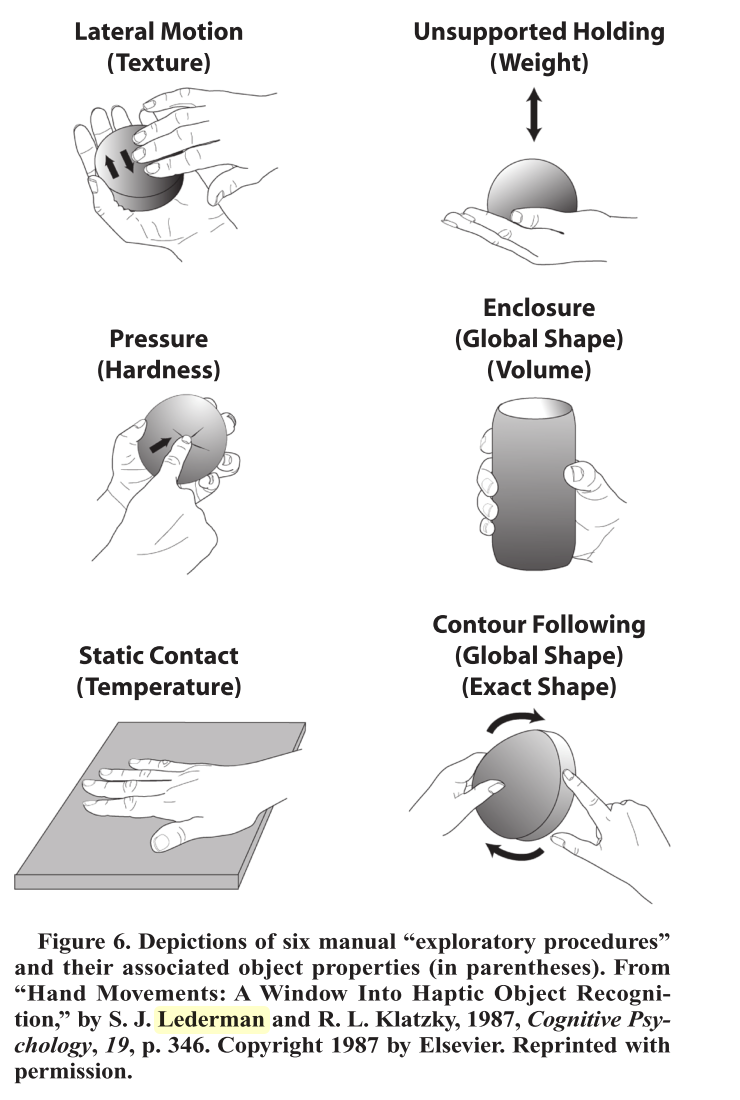
\includegraphics[width=7cm]{1_Bible/Photos/Psychology/proc_explo.png}
	\caption{Procédure d’exploration [] }\label{proc_explo}
\end{figure}


